\documentclass{myhw}
\linespread{1.05}        % Palatino needs more leading (space between lines)
\usepackage{extarrows}
\usepackage{mathrsfs}
\usepackage{braket}
\titleformat{\section}[runin]{\sffamily\bfseries}{}{}{}[]
\titleformat{\subsection}[runin]{\sffamily\bfseries}{}{}{}[]
\renewcommand{\exname}{Question }
\renewcommand{\subexcounter}{(\alph{homeworkSectionCounter})}
\newcommand{\id}{\text{Id}}
\newcommand{\tr}{\text{Tr}}
\newcommand{\rib}{\text{Rib}}

\usepackage{subfigure}

%\usepackage{amsmath}

\title{CSC 2516 Programming Assignment 2}

\begin{document}

%% Question 1
\begin{homeworkProblem}
Colourization as Classification.
\begin{homeworkSection}
Complete the model CNN.
\end{homeworkSection}
\begin{homeworkSection}
\emph{Run main training loop of CNN. This will train the CNN for a few epochs using the cross-entropy objective. It will generate some images showing the trained result at the end. Do these results look good to you? Why or why not?} \\ \\
I don't think the results look good. For the training dataset, although the boundary of objects is basically detected, the objects are still not coloured as the true labels. For the test dataset, the boundary becomes even blurred.
\end{homeworkSection}
\begin{homeworkSection}
\emph{Compute the number of weights, outputs, and connections in the model, as a function of NF and NC. Compute these values when each input dimension (width/height) is doubled. Report all 6 values.}
\begin{center}
\begin{tabular}[h]{ |c|c|c|c| } 
\hline
Layers & Output Units & Weights & Connections \\
\hline
Image & 32*32*1 & - & - \\
MyConv2D-NF & 32*32*NF & 3*3*1*NF=9NF & 9NF*32*32=9216NF \\
MaxPool & 16*16*NF & - & - \\
MyConv2D-2NF & 16*16*2NF & 3*3*NF*2NF=18$\text{NF}^2$ & 18$\text{NF}^2$*16*16=4608$\text{NF}^2$ \\
MaxPool & 8*8*2NF & - & - \\
MyConv2D-2NF & 8*8*2NF & 3*3*2NF*2NF=36$\text{NF}^2$ & 36$\text{NF}^2$*8*8=2304$\text{NF}^2$ \\
MyConv2D-NF & 8*8*NF & 3*3*2NF*NF=18$\text{NF}^2$ & 18$\text{NF}^2$*8*8=1152$\text{NF}^2$ \\
UpSample & 16*16*NF & - & - \\
MyConv2D-NC & 16*16*NC & 3*3*NF*NC=9NF*NC & 9NF*NC*16*16=2304NF*NC \\
UpSample & 32*32*NC & - & - \\
MyConv2D-NC & 32*32*NC & 3*3*NC*NC=9$\text{NC}^2$ & 9$\text{NC}^2$*32*32=9216$\text{NC}^2$ \\
\hline
Total & - & 9NF+72$\text{NF}^2$+9NF$\cdot$NC+9$\text{NC}^2$ & 9216NF+8064$\text{NF}^2$+2304NF$\cdot$NC+9216$\text{NC}^2$ \\
\hline
\end{tabular}
\end{center}
We assume the convolutional kernels are all $3\times3$. \\
The number of weights, outputs, and connections in the model are (9NF+72$\text{NF}^2$+9NF$\cdot$NC+9$\text{NC}^2$), 1024NC, and (9216NF+8064$\text{NF}^2$+2304NF$\cdot$NC+9216$\text{NC}^2$) respectively. \\ \\
when each input dimension (width/height) is doubled, these values are weights=(9NF+72$\text{NF}^2$+9NF$\cdot$NC+9$\text{NC}^2$), outputs=(4096NC), and connections=(36864NF+32256$\text{NF}^2$+9216NF$\cdot$NC+36864$\text{NC}^2$).
\end{homeworkSection}
\begin{homeworkSection}
\emph{Consider an pre-processing step where each input pixel is multiplied element-wise by scalar a, and is shifted by some scalar b. That is, where the original pixel value is denoted x, the new value is calculated y = ax + b. Assume this operation does not result in any overflows. How does this pre-processing step affect the output of the conv net from Question 1 and 2?} \\ \\
The net work has no need to change. \\
Multiplying the input pixels element-wise by scalar a and then shifting them by scalar b will increase the variance of the input data of both training and test set. \\
I did experiments on the image dataset, i.e., I multiplied the training data and validation data by 10 and added them by 10. The loss curves of training dataset are almost the same, while the previous one converged fast a little. However, the loss curve of validation set changed a lot, where the loss curve on modified validation set become fluctuate and hard to converge.
\end{homeworkSection}
\end{homeworkProblem}


%% Question 2
\begin{homeworkProblem}
Skip Connections.
%%% Subquestion 1
\begin{homeworkSection}
Add a skip connection from the first layer to the last, second layer to the second last, etc.
\end{homeworkSection}
%%% Subquestion 2
\begin{homeworkSection}
\emph{Train the model for at least 25 epochs and plot the training curve using a batch size of 100.} \\ \\
The figure of the training curve of U-Net is shown in Figure \ref{fig:curve_unet}. 
\begin{figure*}[h]
\centering
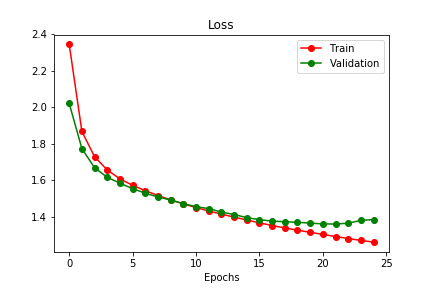
\includegraphics[width=.5\textwidth]{training_curve_unet.png}
\caption{Training curve of U-Net.}
\label{fig:curve_unet}
\end{figure*}
\end{homeworkSection}
\begin{homeworkSection}
\emph{How does the result compare to the previous model? Did skip connections improve the validation loss and accuracy? Did the skip connections improve the output qualitatively? How? Give at least two reasons why skip connections might improve the performance of our CNN models.} \\ \\
The U-Net outperforms the previous network. \\
The skip connections improve the validation loss and accuracy. I trained the both networks with exactly same parameters, and the validation loss and accuracy of the previous network are 1.598 and 40.9\% respectively, while for U-Net they are 1.383 and 48.5\%. \\
The skip connections also improve the output qualitatively (as Figure \ref{fig:results}). The contour of these horses are clearer, and some of the original colors that were not right are corrected by U-Net. 
\begin{figure}[h]
  \centering
  \subfigure[Results on training set of CNN.]{
    \label{fig:train_cnn} 
    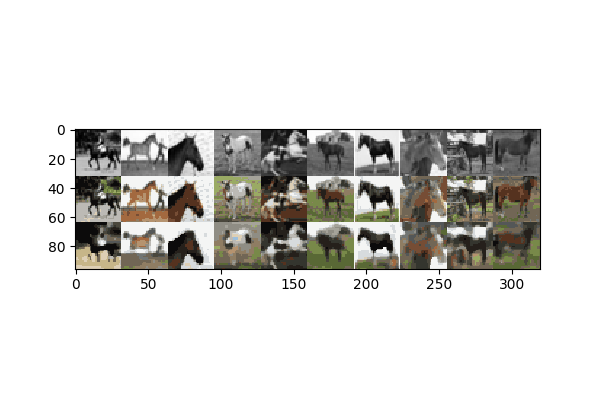
\includegraphics[width=0.47\textwidth,trim=10 60 10 70,clip]{train_24_cnn.png}
  }
%  \hspace{.1in} 
  \subfigure[Results on training set of U-Net.]{
    \label{fig:train_unet} 
    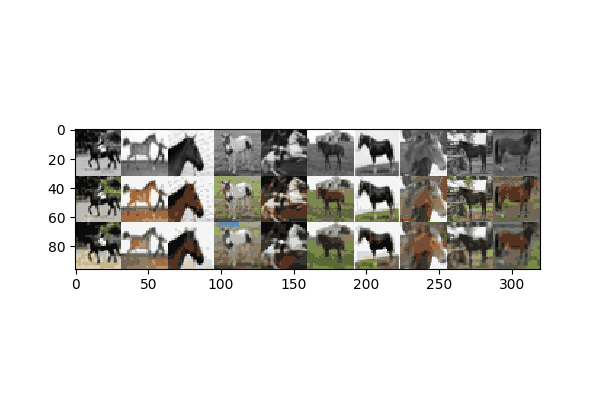
\includegraphics[width=0.47\textwidth,trim=10 60 10 70,clip]{train_24_unet.png}
  } 
  \\
  \subfigure[Results on test set of CNN.]{
    \label{fig:test_cnn} 
    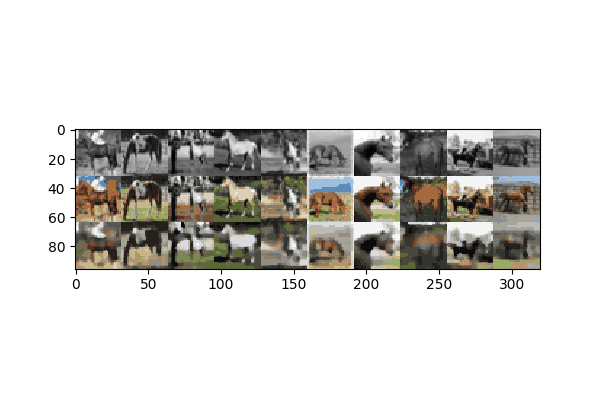
\includegraphics[width=0.47\textwidth,trim=10 60 10 70,clip]{test_24_cnn.png}
  }
%  \hspace{.1in} 
  \subfigure[Results on test set of U-Net.]{
    \label{fig:test_unet} 
    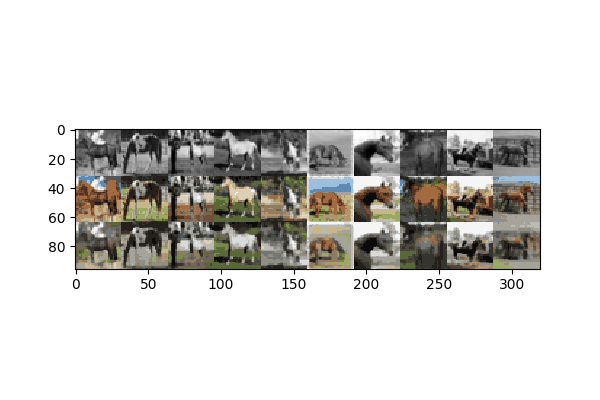
\includegraphics[width=0.47\textwidth,trim=10 60 10 70,clip]{test_24_unet.png}
  }
  \caption{Results of CNN and U-Net networks.}
  \label{fig:results} %% label for entire figure
\end{figure} \\
Two reasons why skip connections might improve the performance of our CNN models:
1) The original CNN reduces the picture size (or no longer corresponds to the input picture size) due to pooling when getting deeper. Compared with the original CNN, the structure of U-Net makes it more accurate for the positioning of each pixel of the picture, and it outperforms CNN to give each pixel its corresponding color value.
2) The deeper layer of U-Net can fully combine the simple representations of the shallow layer, which avoid overfitting, even for small samples.
\end{homeworkSection}
\begin{homeworkSection}
\emph{Re-train a few more “U-Net” models using different mini batch sizes with a fixed number of epochs. Describe the effect of batch sizes on the training/validation loss, and the final image output.} \\ \\
I tested with batch size = 10, 50, 100, 200. \\
The smaller the batch size, the longer the run time. \\
In general, the smaller the batch size, the smaller the loss of the training set. \\
The loss of the test set should also conform to this trend as training set; however, when the batch size becomes small enough (=10), overfitting occurs, as the loss of the test set is not stable. \\
For the final image outputs of different batch size on the test set, when batch size is large, some underfitting occurred, e.g., the contour of the object is not found clearly; however, there are also some deviations when the batch size is too small, such as separating objects (sky, grassland) that should be a whole.
\end{homeworkSection}
\end{homeworkProblem}


%% Question 3
\begin{homeworkProblem}
Fine-tune Semantic Segmentation Model.
\begin{homeworkSection}
Complete the 'train' function to fine-tune only the last layer in our downloaded deeplabv3.
\end{homeworkSection}
\begin{homeworkSection}
Complete the script in Question 2 of Part C by adding around 2 lines of code and train the model.
\end{homeworkSection}
\begin{homeworkSection}
\emph{Visualize the predictions by running the helper code provided.} 
\begin{figure}[h]
  \centering
  \subfigure[Predictions on training set.]{
    \label{fig:trained} 
    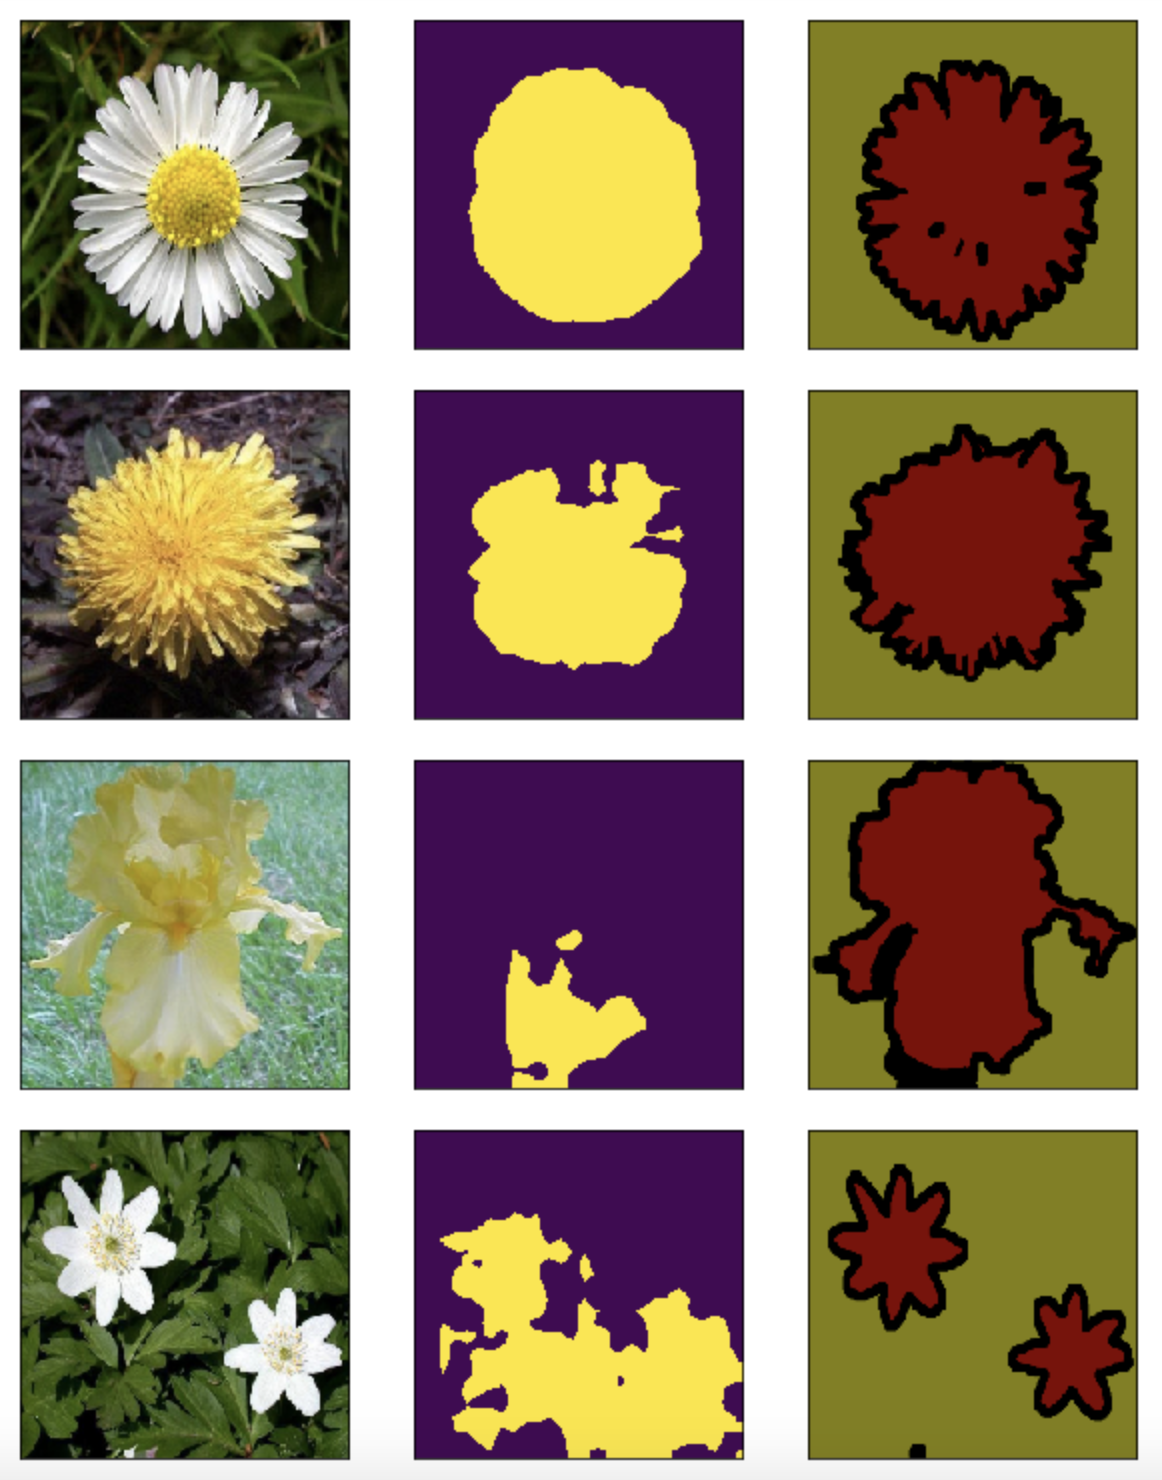
\includegraphics[width=0.4\textwidth]{trained.png}
  }
  \hspace{.3in} 
  \subfigure[Predictions on validation set.]{
    \label{fig:notrained} 
    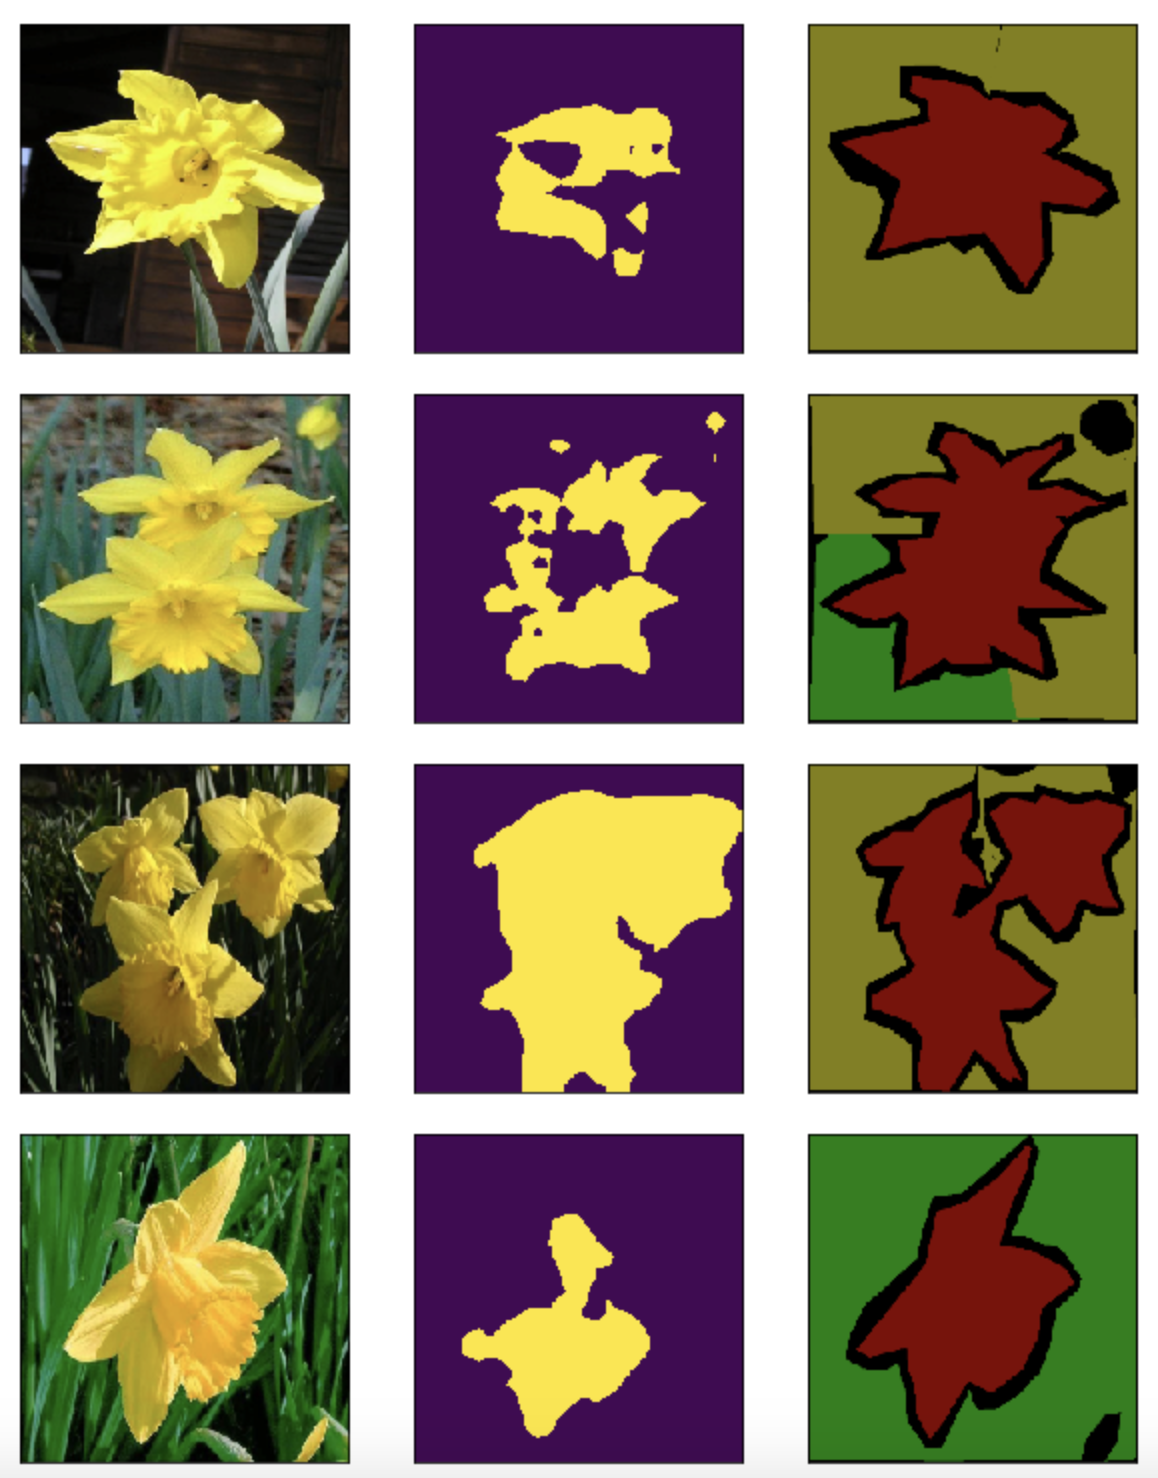
\includegraphics[width=0.4\textwidth]{notrained.png}
  } 
  \caption{Visualization of the predictions of the fine-tuned Semantic Segmentation Model.}
  \label{fig:seg_vis} %% label for entire figure
\end{figure} \\
The visualization of the predictions of the fine-tuned semantic segmentation model is shown in Figure \ref{fig:seg_vis}.
\end{homeworkSection}
\begin{homeworkSection}
\emph{Consider a case of fine-tuning a pre-trained model with n number of layers. Each of the layers have a similar number of parameters, so the total number of parameters for the model is proportional to n. Describe the difference in memory complexity in terms of n between fine-tuning an entire pre-trained model versus fine-tuning only the last layer (freezing all the other layers). What about the computational complexity?} \\ \\
The memory complexity of fine-tuning the entire model is \textbf{n times} that of fine-tuning of the last layer.
We freeze the other layers, so back-propagation does not enter these layers.
It should be noted that in addition to saving parameters, fine-tuning the entire network also needs to save the gradient of the intermediate layer results. \\
The back-propagation computational complexity of fine-tuning the entire model is also n times that of fine-tuning of the last layer. However, freezing the other layers will not decrease the computational complexity of the forward process, which is almost the same as the computational complexity of the backward process. As a result, the computational complexity of fine-tuning the entire model is \textbf{equal} to that of fine-tuning of the last layer, which are both O(n).
\end{homeworkSection}
\begin{homeworkSection}
\emph{If we increase the height and the width of the input image by a factor of 2, how does this affect the memory complexity of fine-tuning? What about the number of parameters?} \\ \\
The height and the width of the input image will affect the memory complexity of fine-tuning. All the intermediate results are stored for computing the next intermediate results. The memory complexity of the intermediate units (such as feature maps) will be increased by the factor of 4, while the memory complexity of the parameters will not change.
\\ 
If the model has no fully connected layers, the number of parameters will not be influenced by the height and the width of the input image.
\end{homeworkSection}
\end{homeworkProblem}

\end{document}

%\begin{gather*}
%\end{gather*}



